% USC EE599 Team 10 -- Final Project Report
% Self-contained academic manuscript. Compile: latexmk -pdf -interaction=nonstopmode main.tex
% Final experimental values transcribed from final(3).md (not new measurements).
\documentclass[10pt,twocolumn]{article}
\usepackage[letterpaper,top=0.68in,bottom=0.68in,left=0.69in,right=0.69in,columnsep=0.24in]{geometry}
\usepackage[T1]{fontenc}
\usepackage[utf8]{inputenc}
\usepackage{newtxtext,newtxmath}
\usepackage{microtype}
\usepackage{graphicx}
\usepackage{amsmath}
\usepackage{booktabs,array,tabularx}
\usepackage[font=small,labelfont=bf,labelsep=period,skip=4pt]{caption}
\usepackage{enumitem}
\usepackage{balance}
\usepackage[numbers,sort&compress]{natbib}
\usepackage[hidelinks]{hyperref}
\usepackage{xcolor}
\definecolor{accent}{HTML}{1B4768}
\hypersetup{pdftitle={Reinforcement Learning for Adaptive Defense in Multi-Agent LLM Systems},
    pdfauthor={Ruiteng Li, Shi He, Congkang Lyu},pdfsubject={USC EE599 Final Project Report}}
\setlength{\parindent}{1em}
\setlength{\parskip}{0pt}
\setlength{\textfloatsep}{7pt plus 1pt minus 1pt}
\setlength{\floatsep}{6pt plus 1pt minus 1pt}
\setlength{\intextsep}{6pt plus 1pt minus 1pt}
\setlength{\abovecaptionskip}{4pt}
\setlength{\belowcaptionskip}{2pt}
\renewcommand{\arraystretch}{1.08}
\setlist[itemize]{leftmargin=1.15em,itemsep=1pt,topsep=2pt,parsep=0pt}
\usepackage{titlesec}
\titlespacing*{\section}{0pt}{9pt plus 1pt}{3pt}
\titlespacing*{\subsection}{0pt}{6pt}{2pt}
\titleformat{\section}{\normalsize\bfseries}{\thesection}{0.55em}{}
\titleformat{\subsection}{\small\bfseries}{\thesubsection}{0.55em}{}
\renewcommand{\bibsection}{\section*{References}}
\title{\vspace{-0.42in}\bfseries\fontsize{15}{17}\selectfont Reinforcement Learning for Adaptive Defense\\[-1pt]
 in Multi-Agent LLM Systems\vspace{-0.07in}}
\author{\normalsize Ruiteng Li \qquad Shi He \qquad Congkang Lyu\\[-1pt]
\small University of Southern California, Department of Electrical and Computer Engineering\\[-1pt]
\footnotesize \texttt{ruitengl@usc.edu} \quad \texttt{shihe@usc.edu} \quad \texttt{congkang@usc.edu}\\[-1pt]
\footnotesize EE599 $\cdot$ Team 10}
\date{}
\begin{document}
\maketitle
\vspace{-0.23in}
\begin{abstract}
\noindent
Messages passed between LLM agents are often treated as trustworthy, even though an attacker may change them in transit. Hash voting across redundant routes can expose such changes, but keeping redundancy high for every message is costly. We built a majority-hash communication layer and a reinforcement-learning controller that adjusts the number of routes using recent voting outcomes and delayed feedback. The two parts were tested at different levels. On 427 MBPP tasks with Qwen2.5-14B, the \emph{static} defense reduced the reported AiTM attack success rate from 100\% to 0\% at $k=3$. In separate multi-attacker \emph{simulations}, price-conditioned QR-DQN exceeded a validation-selected fixed policy by 23.2 percentage points at matched modeled cost 8 in the Waves scenario (95\% bootstrap interval: [18.6, 25.6]). The advantage was smaller, and at one high-cost operating point negative, under independent attackers. Removing delayed receipts also hurt performance substantially. Finally, 12 integration tests passed with the implemented integrity engine and simulated attacks. These results support cost-aware adaptation under our attack assumptions, not yet an end-to-end adaptive LLM deployment.

\end{abstract}
\vspace{-0.08in}

\section{Introduction}
In frameworks such as AutoGen, CAMEL, and MetaGPT, LLM agents collaborate by exchanging instructions, intermediate results, and feedback as text \citep{wu2024autogen,li2023camel,hong2024metagpt}. Surveys of LLM-based autonomous agents also point to the central role of communication in these workflows \citep{wang2024survey,xi2023rise}. That makes the communication link itself worth protecting. An Agent-in-the-Middle (AiTM) attacker can alter one of these messages without touching the underlying models \citep{he2025aitm}. The receiving agent may then act on content that its collaborator never intended to send. Prompt-level safeguards do not, by themselves, tell the receiver whether a message was changed on the way.

Our starting point was a fairly simple defense: send the message over several logical routes and compare hashes by majority vote. A small number of full-payload copies plus lightweight hash witnesses avoids sending the same text everywhere. The difficulty is deciding how much redundancy to buy. A large $k$ may be useful during a burst of attacks, but it is a poor default when the network is quiet. This motivated our central question: \emph{can a controller adjust redundancy from imperfect feedback and achieve better integrity success at the same average communication cost?}

We investigate this with an implemented hash-voting layer, a synthetic multi-attacker environment, and a price-conditioned QR-DQN controller. We also compare learned policies with fixed routing, tuned rules, and supervised predictors rather than treating RL as the only reasonable option. There is an important boundary to the evidence: the live-LLM benchmark tests the static defense, whereas the dynamic controller is evaluated in simulation. We keep those results separate throughout the paper.

\subsection{Related work}
Prior studies have investigated attacks on multi-agent collaboration and debate \citep{amayuelas2024collaboration}, communication-level AiTM manipulation \citep{he2025aitm}, and agent malfunction amplification \citep{zhang2024breaking}. Work on inter-agent consistency in debates \citep{xiong2023consistency} raises a related reliability question, but our focus is specifically on whether the message arriving over a route has been altered. The majority-vote rule is related to classical Byzantine fault tolerance \citep{lamport1982byzantine}; its role in LLM multi-agent reliability has also been discussed \citep{zheng2025bft}. Here we compare hashes of one transmitted payload, not independently generated agent outputs. Moving-target defense has been explored at the network level \citep{skowyra2020mtd} and for LLM security \citep{chen2023jailbreaker}; our changing resource is the number of hash-verification routes. RL-based cyber defense has likewise addressed security expenditure versus attack loss \citep{nyberg2023defense}. We test whether past integrity feedback supports better redundancy choices than a strong fixed-cost baseline.

\begin{figure*}[t]
\centering
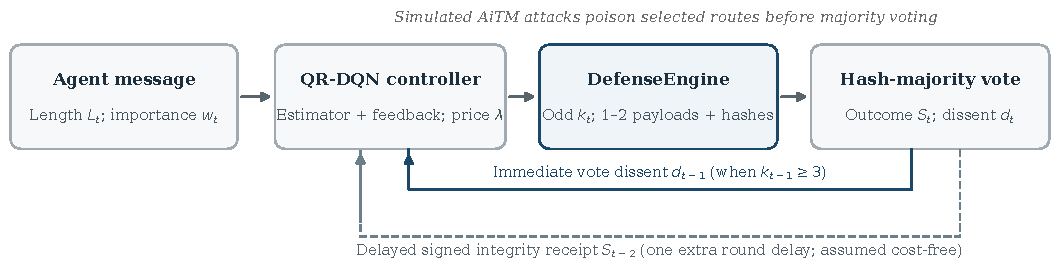
\includegraphics[width=0.965\textwidth]{figures/architecture.pdf}
\caption{Integrated design. A sender's message is protected by a hash-majority engine with redundancy $k$ selected by a price-conditioned controller. The attacker and closed-loop feedback are simulated in the final integration test; a live LLM is used only in the separate static experiment.}
\label{fig:architecture}
\end{figure*}

\section{Threat Model and Integrity Engine}
\subsection{Communication-layer verification}
We assume an attacker can modify transmissions on a subset of logical routes between two otherwise benign agents. For a message $m$ of $L$ bytes, the sender hashes the payload as $H(m)$ and chooses an odd $k\in\{1,3,\ldots,101\}$. The first two routes, when present, carry the payload and its hash; further routes send only 64-byte hash witnesses. This asymmetric design saves bytes compared with replicating the entire payload $k$ times. The receiver uses a strict majority over the received hashes. When $n_t$ routes carry the same attacker-chosen hash, the simulator marks the round successful exactly when

\begin{equation}\label{eq:success}
S_t=\mathbb{1}\big[n_t\leq(k_t-1)/2\big].
\end{equation}
A strict honest majority prevents the poisoned hash from winning \citep{lamport1982byzantine}. But this is a \emph{hash-integrity} result, not a delivery guarantee. Both full-payload routes could be unavailable or corrupted even while enough witnesses preserve the correct hash. Our metric therefore does not establish that an intact message reaches the receiving agent. We also do not evaluate hash collisions or attacks on the feedback channel.

The modeled bytes and normalized relative cost are
\begin{equation}\label{eq:cost}
\begin{split}
B(k,L)&=\min(k,2)L+64\max(0,k-2),\\
c(k,L)&=B(k,L)/\max(128,2L).
\end{split}
\end{equation}
The cost $c$ measures modeled bytes relative to a two-payload reference; it is not measured throughput or latency. The $k=1$ case keeps its single payload in the numerator. Unlike the earlier milestone prototype, the final controller cannot retry a failed transmission, and we no longer use the milestone's 164-byte incremental cost reference. This matters when reading the older results alongside the present ones.

\subsection{Dynamic synthetic adversaries}
Real AiTM traces were not available for this evaluation. We instead use a three-stage attacker model---quiet, probing, and burst---following the hidden-state modeling approach of \citet{liao2020hmm}. Each attacker changes stage according to the \emph{chosen}, not data-fitted, transition matrix

\begin{equation}\label{eq:hmm}
P=\begin{bmatrix}.90&.09&.01\\ .10&.75&.15\\ .05&.10&.85\end{bmatrix},\quad
p_{\rm attack}=(.02,.20,.75).
\end{equation}
When an attacker acts, it compromises $\min\{3,1+\operatorname{Poisson}(\mu_z)\}$ routes, with $\mu_z\in\{0,0.5,2\}$ for the three stages. We set compromise persistence to 0.72, limit concurrent compromise to 50 routes, and vary the attacker population between 0 and 40. All compromised routes use the same poisoned hash in a round. Table~\ref{tab:scenarios} shows the four conditions: independent attackers, sudden population changes, coordinated campaigns, and their combination. For Waves, the attacker count jumps with probability 0.03 each round, multiplied by one of $\{0.4,0.6,1.6,2.5\}$. Campaign uses 0.70 coupling to a shared stage. None of these numbers should be read as measured attack frequencies.

\begin{table}[t]
\centering
\caption{Final synthetic attack scenarios. Coupling and population jumps are injected by the simulator; they are not fitted attack statistics.}
\label{tab:scenarios}
\footnotesize
\setlength{\tabcolsep}{3.6pt}
\begin{tabular}{@{}p{.31\columnwidth}p{.57\columnwidth}@{}}
\toprule
Scenario & Temporal dependence \\
\midrule
Independent & 20 attackers; separate HMM stages \\
Waves & 0--40 attackers; 3\% population-jump probability per round \\
Campaign & 20 attackers; 70\% shared-stage coupling \\
Campaign + waves & Shared stages and population jumps \\
\bottomrule
\end{tabular}
\end{table}

\section{Cost-Aware Adaptive Controller}
The controller does not know how many routes will be compromised in the current round. It sees message length $L_t\in\{50,100,200\}$, importance $w_t\in\{0.5,1,1.5\}$, the price $\lambda$, earlier voting disagreements (when $k\geq3$), and a receipt reporting the preceding round's integrity result. An estimator uses the votes and receipts to infer the earlier compromise count when possible, or a lower bound otherwise. Its 22 features include exponential moving averages with rates 0.5, 0.2, and 0.05. The hidden attacker stages, attacker count, and current compromise total remain unavailable. We assume the one-round-delayed receipt is trustworthy and has no communication charge; that is a significant simplification, examined later.

We did not ask the RL agent to choose from every possible odd $k$ directly. It has 19 actions: twelve explicit values $\{1,3,5,7,9,13,17,21,27,35,45,61\}$ and seven margins $a\in\{-1,0,0.5,1,1.5,2,3\}$ around the estimated compromise count $\hat n_t$. A margin is converted into an admissible odd $k$ through

\begin{equation}\label{eq:action}
 k_t=\operatorname{clip}_{\mathcal K}\!\left(2\left\lceil\hat n_t+a\sqrt{\hat n_t+1}\right\rceil+1\right).
\end{equation}
We reward correct hash-majority outcomes, penalize failures more heavily, and charge for transmitted bytes:

\begin{equation}\label{eq:reward}
r_t=w_t\big[S_t-1.65(1-S_t)\big]-\lambda c(k_t,L_t).
\end{equation}
The price $\lambda$ is part of the observation, so changing it at test time traces a success--cost curve without retraining for each budget. It is sampled log-uniformly from $[0.01,5]$ during training. We use QR-DQN \citep{dabney2018qrdqn} with a $64\times64$ two-hidden-layer network, 50 quantiles, discount 0.95, learning rate $3\times10^{-4}$, replay capacity 200k, batch size 256, and 600k training steps. Three training seeds (2026--2028) support the main results. Figure~\ref{fig:architecture} sketches the engine and feedback loop.

\subsection{Training choices and changes since the milestone}
The QR-DQN policy is trained primarily with Campaign + waves attacks, but we deliberately vary the environment. Campaign coupling is switched off in 35\% of training episodes and population waves in 40\%, exposing the policy to more independent-like conditions. Following 8,000 random steps, $\epsilon$-greedy exploration decreases from 1 to 0.04 over the first 30\% of the 600k-step run. We take two gradient steps every four environment steps and update the target network every 2,000 steps. The aim is for the policy to respond to signals it could actually observe, not to hidden state available only inside the simulator.

Our earlier milestone used $k\in\{1,3,5,7\}$ with one possible retry. For the final study we removed retries, expanded the available redundancy levels, changed the cost definition, and used longer episodes and a different evaluation protocol. The old and new success--cost curves are not numerically interchangeable. We retain the earlier static LLM benchmark only as separate evidence for the communication defense.

\section{Experimental Protocol}
\subsection{Evaluation and comparisons}
Each simulated episode contains 256 messages. We evaluate on 20 held-out seeds (1000--1019) across four attack scenarios. RL controllers are evaluated at 16 prices and supervised methods at eight. Our two reported quantities are importance-weighted hash-majority success and average modeled byte cost:

\begin{equation}\label{eq:metric}
\hat p=\frac{\sum_{e,t}w_{e,t}S_{e,t}}{\sum_{e,t}w_{e,t}},\qquad \bar c=\frac{1}{N}\sum_{e,t}c(k_{e,t},L_{e,t}).
\end{equation}
We put particular care into the fixed baseline. It can select any of the 51 odd redundancy values and randomly mix adjacent values to reach intermediate mean costs. We first determine its best success--cost frontier on validation seeds 3000--3019 and then \emph{freeze} that selection before using test seeds. This avoids choosing the best fixed policy after looking at test outcomes. Policies are compared at the same observed $\bar c$ by interpolation within measured cost ranges; we do not extrapolate. The reported gain $\Delta_\pi(c)=100[\hat p_\pi(c)-\hat p_{\rm fixed}(c)]$ is in percentage points. Pointwise 95\% intervals come from 500 bootstrap resamples of the 20 test seeds, not from repeated draws of the HMM parameters.

Other comparisons include a six-parameter rule tuned over 150 random configurations, eight supervised models using 60k oracle-labeled samples, and DQN, PPO, A2C, and RecurrentPPO \citep{mnih2015dqn,schulman2017ppo}. Where applicable, methods have access to the same observation information. Only the primary QR-DQN experiment uses three training seeds; alternative RL methods and ablations use one seed (2026), limiting claims about algorithm rankings.

\begin{figure*}[t]
\centering
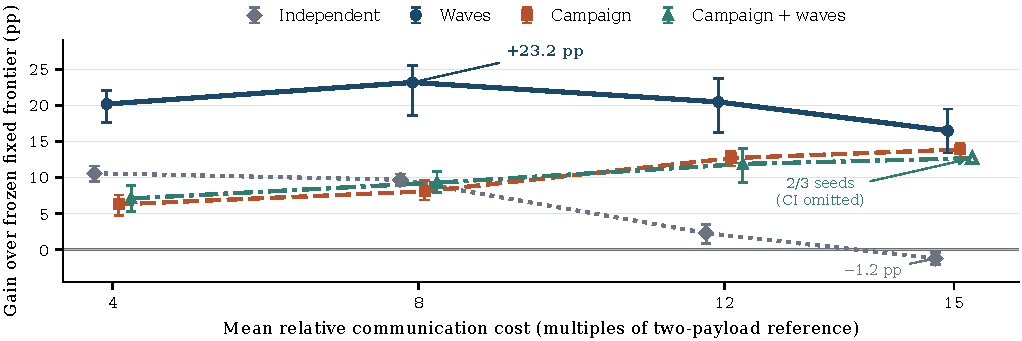
\includegraphics[width=.975\textwidth]{figures/main_gain.pdf}
\caption{Principal result: QR-DQN (average over three training seeds) minus the validation-selected fixed frontier at matched actual communication cost. Markers show reported percentage-point gains; whiskers are pointwise 95\% bootstrap intervals from 20 test seeds (500 resamples). Campaign + waves at cost 15 has coverage from two of three training seeds. Shown points are directly reported values, connected only as a visual guide.}
\label{fig:gain}
\end{figure*}

\section{Results and Analysis}
\subsection{Static LLM test and engine integration}
The clearest test of the communication layer itself uses a Coder/Reviewer pair with Qwen2.5-14B. Across 427 MBPP tasks \citep{austin2021mbpp}, the reported AiTM attack success rate fell from 100\% without defense to 0\% with $k=3$, while reported system availability stayed at 100\%. This experiment involves a real LLM, but \emph{does not} test the learned controller.

For the final integration demo, we connected the implemented \texttt{DefenseEngine} to simulated attackers and fixed, rule-based, or QR-DQN controllers. In all 18 reported scenario--policy combinations, the engine outcome agreed with Eq.~\eqref{eq:success}; all 12 integration tests passed, including the byte-accounting and observation checks. We view this as a consistency check between code and simulator, rather than evidence for a live adaptive LLM system.

\begin{table}[t]
\centering
\caption{Observed importance-weighted success of the \emph{frozen fixed baseline} at matched costs, before subtracting it from any adaptive score. Values are fractions, not percentage-point gains.}
\label{tab:fixed}
\footnotesize
\setlength{\tabcolsep}{3.5pt}
\begin{tabular}{@{}lrrrr@{}}
\toprule
Scenario & $c{=}4$ & $c{=}8$ & $c{=}12$ & $c{=}15$\\
\midrule
Independent & .250 & .533 & .816 & .954\\
Waves & .231 & .439 & .630 & .755\\
Campaign & .412 & .583 & .661 & .718\\
Campaign + waves & .515 & .673 & .758 & .794\\
\bottomrule
\end{tabular}
\end{table}

\subsection{Where adaptation helps---and where it does not}
The largest difference in Fig.~\ref{fig:gain} is under Waves. At modeled cost 8, QR-DQN improves on the frozen fixed frontier by \textbf{23.2 pp} (95\% CI [18.6,25.6]); even at cost 15 it retains a 16.5 pp gain [13.4,19.5]. At cost 8, the improvements in Independent, Campaign, and Campaign + waves are 9.7 [8.9,10.5], 8.1 [6.9,9.6], and 9.3 pp [7.9,10.8], respectively. Sudden changes in attacker population give recent feedback more value: a single fixed $k$ has to compromise between quiet and severe rounds.

There is also a useful counterexample. For Independent attackers at cost 15, QR-DQN is \textbf{1.2 pp below} the fixed frontier (95\% CI [--2.0,--0.4]). The fixed policy is already successful in 95.4\% of weighted rounds at that cost (Table~\ref{tab:fixed}), so there is little room left for improvement. We would not claim that RL is uniformly preferable. The tuned heuristic also performs well: in Waves at cost 15 its reported gain is 17.3 pp, slightly above QR-DQN's three-seed average of 16.5 pp. These results point to the value of \emph{adaptive feedback use}, which does not necessarily require a neural policy.

\begin{table}[t]
\centering
\caption{RL algorithm comparison at matched modeled cost 8, gain over frozen fixed baseline (pp). \emph{Single training seed 2026 for every entry}; descriptive only.}
\label{tab:rl}
\footnotesize
\setlength{\tabcolsep}{4.2pt}
\begin{tabular}{@{}lrrr@{}}
\toprule
Scenario & QR-DQN & DQN & PPO\\
\midrule
Independent & +11.8 & +7.6 & +11.6\\
Waves & +23.2 & +21.2 & +25.4\\
Campaign & +8.7 & +6.3 & +8.3\\
Campaign + waves & +9.8 & +8.7 & +10.3\\
\bottomrule
\end{tabular}
\end{table}

\subsection{How the pattern changes with budget}
The four scenarios do not share one simple trend. In Independent, the gain shrinks from 10.6 pp at cost 4 to 2.3 pp at cost 12, before turning negative at cost 15. Waves stays positive at each plotted budget: 20.2, 23.2, 20.5, and 16.5 pp at costs 4, 8, 12, and 15. Campaign moves in the opposite direction, from 6.3 pp at cost 4 to 13.9 pp at cost 15. Campaign + waves increases from 7.1 to 11.9 pp between costs 4 and 12. Its reported 12.7 pp gain at cost 15 uses only two training seeds because the third seed did not reach that cost. We therefore avoid treating every plotted endpoint as equally supported. A policy that looks best at cost 8 may not be the right choice at cost 15.

\subsection{Other learners and ablation studies}
At cost 8, QR-DQN, DQN, and PPO all outperform the fixed frontier in the single-seed comparison (Table~\ref{tab:rl}). Their numbers are close enough that we cannot rank them confidently with one training run each. A2C mostly chose a cost near 0.46 (roughly $k=1$), and RecurrentPPO remained near 1.27. Neither produced a useful price-dependent curve within 600k steps. This is a limitation of these training runs, not proof that the algorithms would fail after retuning.

We also tried eight supervised predictors: Gaussian Naive Bayes, Logistic Regression, Linear SVM, Decision Tree, Random Forest, Extra Trees, Histogram Gradient Boosting, and an MLP. They learned from single-round optimal-$k$ labels computed using the simulator's true compromise count, but that count was \emph{not} supplied at deployment time. Validation accuracy ranged from about 0.31 to 0.51. At Independent cost 8, Decision Tree, Histogram Gradient Boosting, Linear SVM, and Gaussian Naive Bayes fell below fixed routing by 10.5, 16.2, 15.6, and 27.5 pp. One exception was Histogram Gradient Boosting at Waves cost 4 (+4.0 pp, CI [1.0,6.4]); it still trailed single-seed QR-DQN (+20.8 pp). Several methods did not cover certain target costs, so they cannot be compared at those points. It seems possible that single-round labels are a poor fit for the sequential, price-aware problem, but we did not run a controlled test of that explanation.

\begin{figure}[t]
\centering
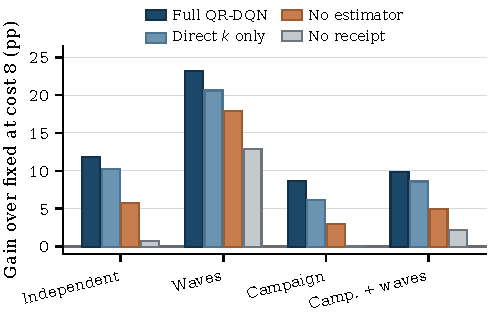
\includegraphics[width=\columnwidth]{figures/ablation.pdf}
\caption{QR-DQN ablations at cost 8 (one training seed, 2026). Each series is the gain over the same frozen fixed baseline; no cross-seed uncertainty is available.}
\label{fig:ablation}
\end{figure}

The ablations in Fig.~\ref{fig:ablation} tell us more about \emph{which information is useful} than about which network architecture wins. At cost 8, removing the one-round-delayed receipt changes the Waves gain from 23.2 to 12.9 pp, Campaign from 8.7 to 0.1 pp, and Campaign + waves from 9.8 to 2.2 pp. Hiding the estimated attack-count features leaves gains of 17.9, 3.0, and 5.0 pp in those scenarios. Using direct $k$ actions only gives 20.6, 6.2, and 8.6 pp. The receipt has a particularly large effect in these runs, but it is assumed cost-free and trustworthy, and each ablation has only one training seed.

\subsection{A useful check with a tuned rule}
A non-neural rule is an important comparison here: if a small hand-designed controller makes the same choices, the contribution may be feedback rather than deep learning. The six-parameter rule ablations in Table~\ref{tab:rule} suggest exactly that. Averaged over the four scenarios at cost 12, dropping receipts changes its gain from 8.7 to 2.6 pp; dropping message length and importance changes it to 6.7 pp. Each version was re-tuned with a separate random search, so one- or two-point differences are not strong evidence on their own.

\begin{table}[t]
\centering
\caption{Tuned rule ablations: gains over fixed frontier, averaged across four scenarios (pp). Separate random-search tuning for each variant.}
\label{tab:rule}
\footnotesize
\setlength{\tabcolsep}{4.2pt}
\begin{tabular}{@{}lrrr@{}}
\toprule
Rule configuration & Cost 4 & Cost 8 & Cost 12\\
\midrule
Full tuned rule & +2.4 & +4.7 & +8.7\\
No message-value feature & +1.1 & +3.4 & +6.7\\
No receipt & +4.8 & +4.0 & +2.6\\
Receipt delay 2 rounds & +3.8 & +5.1 & +7.8\\
\bottomrule
\end{tabular}
\end{table}

One integration example puts these comparisons in perspective. In Campaign + waves, fixed $k=33$ achieved mean cost 11.7 and success 0.724, QR-DQN at price 0.05 achieved 12.6 and 0.876, and the tuned rule achieved 12.2 and 0.832. These are \emph{not matched costs}; the demo used only six seeds and a few fixed choices. We include it to show the real engine and controller can run together, not as an additional claim that QR-DQN wins a fair performance comparison.

\section{Limitations and Future Work}
\textbf{The attacker model is synthetic.} Its HMM transitions, population jumps, shared stages, and compromise limits were selected for experiments rather than estimated from attacks in the wild. The attacker also does not learn against the defender. Results could change with a different transition matrix or a strategic adversary. Parameter sweeps and trace-informed tests are needed before extrapolating beyond these four scenarios.

\textbf{Hash agreement is not message delivery.} We count a correct winning hash, even if no intact full payload is available to the agent. We do not measure downstream task success or denial-of-service behavior in the dynamic runs. The sender's reference hash and the receipt channel are trusted in the simulator; in reality a secure receipt needs bandwidth, authentication, and error handling. Since removing receipts had such a large effect, that deployment cost should be measured rather than ignored.

\textbf{The evidence is still limited.} The static MBPP test uses live LLM agents, but the adaptive closed loop has only been exercised with simulated attackers. The main QR-DQN comparison averages three training seeds; other methods and ablations have one. The bootstrap intervals resample 20 test seeds and omit variability from training and the attack-model assumptions. We cannot infer real-world reliability from those intervals alone.

\subsection{Next experiment: closing the loop with live agents}
A natural next step is to run the learned controller in the same live Coder/Reviewer workflow used for the static defense, but with attacks changing over time. We would measure not only hash-majority correctness, but also whether the receiver actually obtains an intact message, whether poisoned instructions alter the task outcome, and how much the extra routes and receipts cost in real bytes and latency. A malicious network may delay, replay, or suppress feedback, so receipt authentication and failure behavior should be part of that test. Fixed, tuned-rule, and learned policies should then be compared at the same \emph{measured} communication budget. We would also repeat training with more seeds and test additional models and workloads.

\section{Conclusion}
Our experiments suggest that redundancy is worth adapting when attacks have recognizable changes over time. We implemented a lightweight majority-hash layer, tested its static protection on 427 live-LLM coding tasks, and evaluated adaptive route selection in a separate multi-attacker simulator. QR-DQN gained as much as 23.2 pp over the frozen fixed baseline under Waves, but did not win everywhere. The receipt ablations and tuned-rule results point to useful feedback as a key ingredient. What remains open is whether that advantage survives real agent workflows, imperfect receipts, and measured network costs.

\noindent\textbf{Team contributions.} Ruiteng Li developed the communication-layer verification and integration; Shi He developed attack modeling and adaptive controllers; Congkang Lyu led matched-cost evaluation, uncertainty analysis, and visualizations. All three contributed to the report.

% The instructor excludes references from the six-page body limit.
% Force bibliography onto a new page so the body-page count is directly auditable.
\clearpage
\balance
\bibliographystyle{unsrtnat}
\bibliography{references}
\end{document}
